
%(BEGIN_QUESTION)
% Copyright 2005, Tony R. Kuphaldt, released under the Creative Commons Attribution License (v 1.0)
% This means you may do almost anything with this work of mine, so long as you give me proper credit

Calculate all voltage drops and currents in this circuit, complete with arrows for current direction and polarity markings for voltage polarity.  Then, calculate the overall voltage gain of this amplifier circuit ($A_V$), both as a ratio and as a figure in units of decibels (dB):

$$\includegraphics[width=15.5cm]{i01475x01.eps}$$

\vskip 20pt \vbox{\hrule \hbox{\strut \vrule{} {\bf Suggestions for Socratic discussion} \vrule} \hrule}

\begin{itemize}
\item{} Identify the ``simplifying assumptions'' we generally use when analyzing DC opamp circuits.  Hint: one has to do with the effect of negative feedback on the input voltages, and another has to do with the input terminal currents.
\item{} Explain how this circuit would respond if the 22 k$\Omega$ resistor failed open.
\item{} Explain how this circuit would respond if the 22 k$\Omega$ resistor failed shorted.
\item{} Explain how this circuit would respond if the 47 k$\Omega$ resistor failed open.
\item{} Explain how this circuit would respond if the 47 k$\Omega$ resistor failed shorted.
\item{} Explain how this circuit would respond if the (+) and ($-$) opamp inputs were swapped.
\end{itemize}

\underbar{file i01475}
%(END_QUESTION)





%(BEGIN_ANSWER)

$$\includegraphics[width=15.5cm]{i01475x02.eps}$$

$A_V$ = 0.468 = -6.594 dB

%(END_ANSWER)





%(BEGIN_NOTES)

Operational amplifier circuits provide a great opportunity to review basic concepts of DC circuits: voltage drops, polarity, current directions, Ohm's Law, Kirchhoff's Voltage Law, Kirchhoff's Current Law, etc.  This circuit is no exception.  Emphasize the fact that a great many opamp circuits may be comprehensively analyzed merely with knowledge of these fundamental principles and the characteristics of an ideal opamp (zero input current, infinite open-loop gain, unlimited output voltage swing, zero voltage between input terminals when negative feedback is in effect).

Some students may arrive at the wrong gain figure because they blindly followed a formula with $R_1$ and $R_2$ shown as variables, plugging in this circuit's values for $R_1$ and $R_2$ without considering which resistor is which (is $R_1$ the feedback resistor or is $R_2$?).  This is by design, as I want students to learn to {\it think} about what they are doing rather than thoughtlessly follow instructions.





\vfil \eject

\noindent
{\bf Summary Quiz:}

Calculate the amount of current through resistor $R_1$ in this op-amp circuit:

$$\includegraphics[width=15.5cm]{i01475x03.eps}$$

\begin{itemize}
\item{} 0.812 mA
\vskip 5pt 
\item{} 0.628 mA
\vskip 5pt 
\item{} 11.6 mA
\vskip 5pt 
\item{} 6.21 mA
\vskip 5pt 
\item{} 2.70 mA
\vskip 5pt 
\item{} 8.91 mA
\end{itemize}


%INDEX% Electronics review: opamp inverting amplifier circuit

%(END_NOTES)


